\documentclass[times, utf8, zavrsni]{fer}

\usepackage{booktabs}
\usepackage[hidelinks]{hyperref}
\usepackage{pdfpages}
\usepackage{float}

\floatstyle{plaintop}
\restylefloat{table}

\begin{document}

\thesisnumber{1205}
\title{Vizualizacija OT elemenata trafostanice opisane jezikom SCL}
\author{Marko Miljković}

\maketitle

% Ispis stranice s napomenom o umetanju izvornika rada. Uklonite naredbu \izvornik ako želite izbaciti tu stranicu.
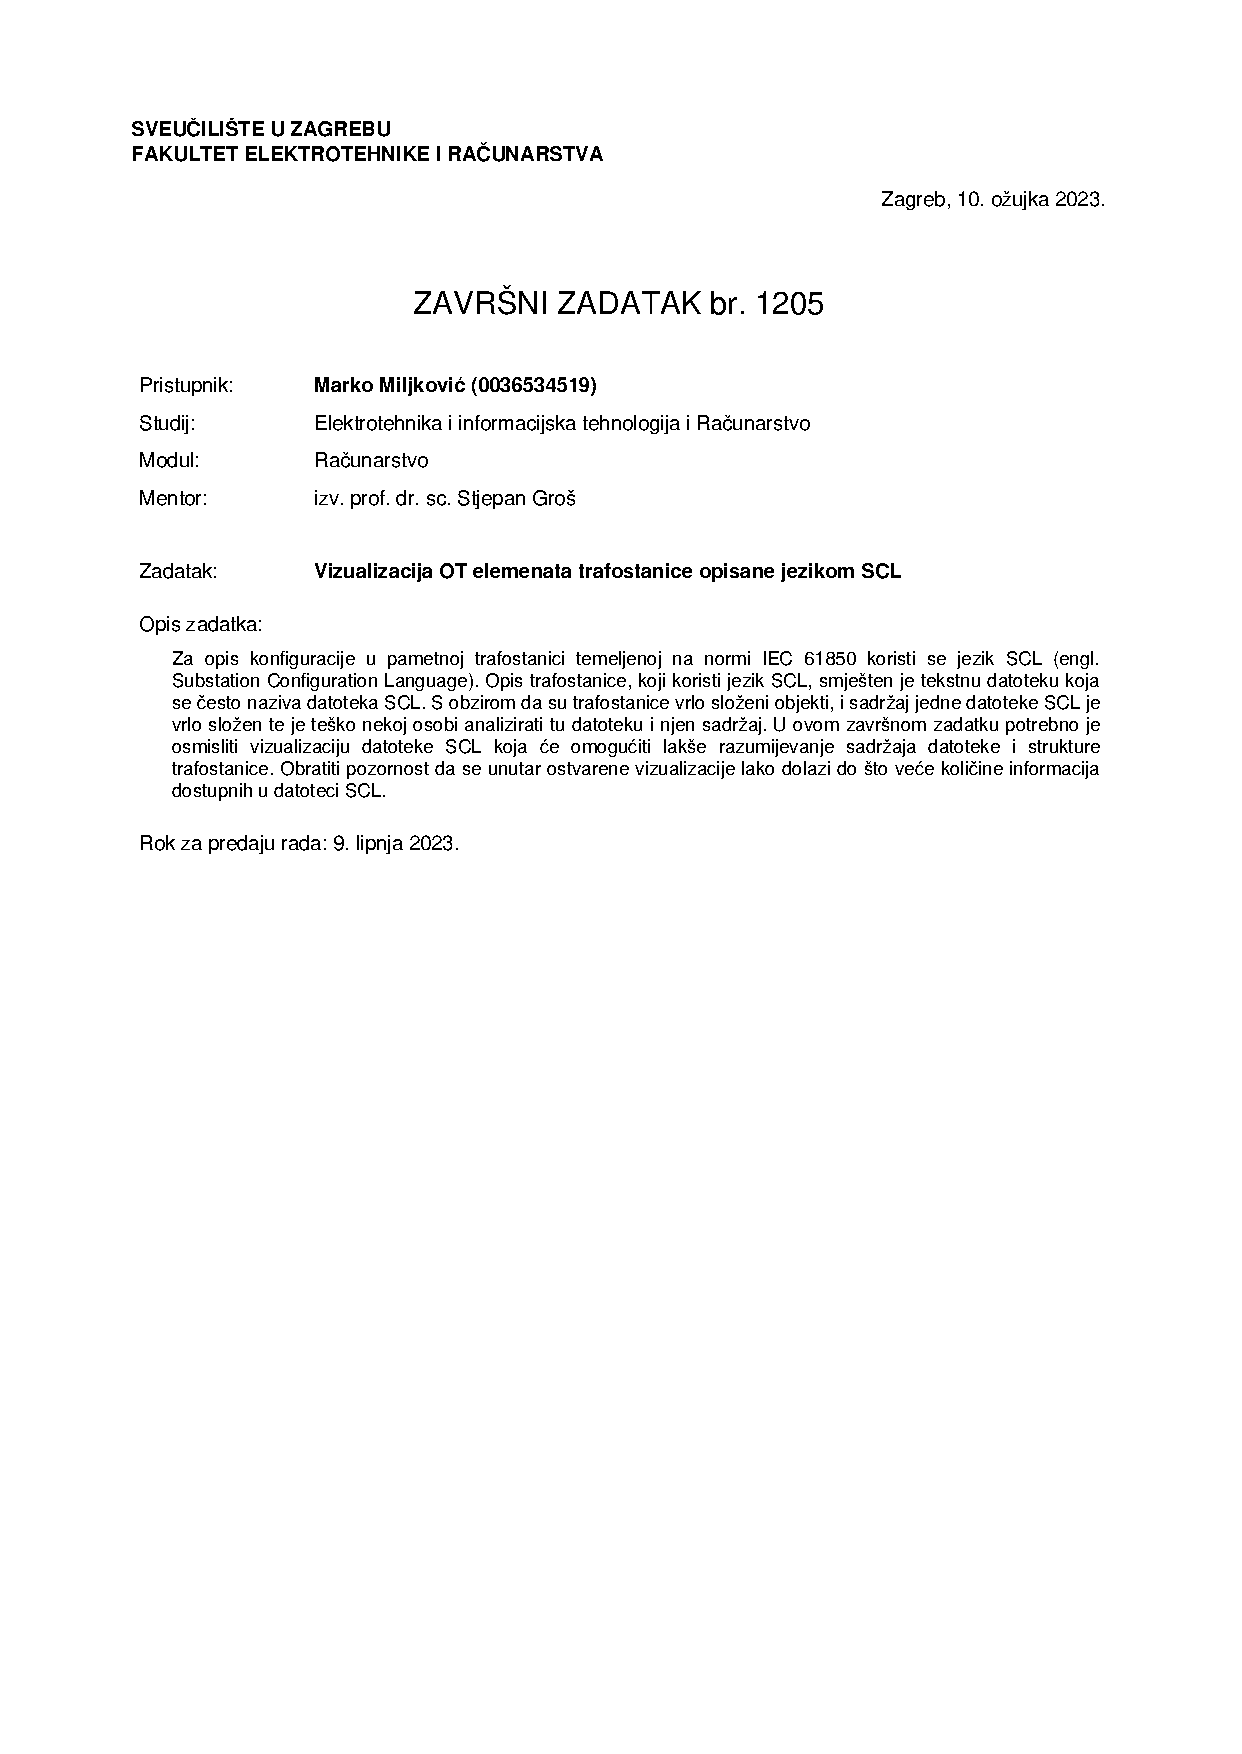
\includepdf[pages=-]{zadatak}

% Dodavanje zahvale ili prazne stranice. Ako ne želite dodati zahvalu, naredbu ostavite radi prazne stranice.
\zahvala{}

\tableofcontents

\chapter{Uvod}
Konfiguriranje trafostanice je težak i kompleksan proces koji je neophodan korak u dostavljanju električne energije kućanstvima. Jedna trafostanica sastoji se od mnoštva sklopki, senzora i raznih drugih električnih uređaja. Svi ti uređaji moraju međusobno komunicirati u stvarnom vremenu.

Standard IEC 61850 razvijen je kako bi se standardizirali podatkovni modeli i komunikacijski protokoli u trafostanicama. Time je pojednostavljen proces konfiguracije uređaja u trafostanicama te je omogućena interoperabilnost uređaja različitih proizvođača.

Ovaj rad se bavi IEC61850 standardom i SCL jezikom kojeg on definira. SCL jezik se koristi za izradu konfiguracijskih datoteka uređaja u trafostanicama, ali za razumijevanje što točno te konfiguracijeske datoteke opisuju morat ćemo ući dublje u IEC 61850 standard. Također će se implementirati vizualizator koji će olakšati analizu konfiguracijskih datoteka.

\bigskip
Drugo poglavlje daje kratak pregled nastanka IEC 61850 standarda i njegovog sadržaja. U trećem poglavlju opisan je model podataka kojeg IEC 61850 standard definira, skupovi podataka i kako se izvješćuju promjene nad tim skupovima podataka. Četvrto poglavlje bavi se abstraktnim komunikacijskim sučeljem IEC 61850 standarda te protokolima na koje se ono preslikava. U petom poglavlju se opisuju različite SCL datoteke i način na koji se one generiraju. U šestom poglavlju su prikazani rezultati implementacije vizualizatora SCL datoteka.

\chapter{Pregled IEC 61850 standarda}
U doba ranih trafostanica 1930-ih godina operateri su koristili telefone kako bi razmjenjivali informacije. Kako se razvijala digitalna mrežna oprema, trafostanice su počele kositriti različite sustave za prikupljanje podataka. Ti sustavi su zbog niske propusnosti mreže koristili posebne protokole specifične za pojedine uređaje kako bi se optimizirala uporaba mreže. To je otežalo konfiguraciju i održavanje takvih sustava.

Rastući broj inteligentnih električnih uređaja \engl{Intelligent Electronic Device, IED} u trafostanicama stvorio je potrebu za definiranjem standarda. Napretkom mrežne opreme i povećanjem propusnosti mrežnih kanala otvorila se mogućnost za razvijanje fleksibilnijeg protokola. Razvoj takvog standarda započeo je 1988., a konačni rezultat bio je IEC 61850 standard za komunikacijske mreže i sustave u trafostanicama. On je unificirao model podatka i komunikacijske protokole u trafostanicama \citep{baigent2004iec}.

\section{Sadržaj}
Standard se sastoji od 10 poglavlja prikazanih u Tablici \ref{tab:iec-chapters}. Poglavlje 6 definira jezik za konfiguraciju trafostanica \engl{Substation Configuration Language, SCL} zasnovan na XML-u.  Poglavlje 7 se bavi stvaranjem apstraktnog modela podataka i apstraktnih sučelja koja će razbiti ovisnost između fizičkih uređaja i konkretnih protokola. Također je uvedena ideja zajedničkih podatkovnih razreda \engl{Common Data Classes, CDC} koji čine građevne jedinice za modeliranje složenijih objekata. U poglavljima 8 i 9 se razmatra preslikavanje apstraktnih sučelja iz poglavlja 7 na konkretne protokole. Poglavlje 10 opisuje proces ispitivanja usklađenosti s IEC 61850 standardom.

\begin{table}[tph]
    \centering
    \begin{tabular}{ |r|l| } 
        \hline
        1. & Uvod i pregled \\ 
        \hline
        2. & Riječnik pojmova \\ 
        \hline
        3. & Opći zahtjevi \\ 
        \hline
        4. & Sustavi i upravljenje projektima \\ 
        \hline
        5. & Komunikacijski zahtjevi za funckije i modele uređaja \\ 
        \hline
        6. & Konfiguracijski jezik vezan za komunikaciju IED uređaja u električnim \\
           & trafostanicama \\ 
        \hline
        7. & Osnovna komunikacijska struktura za trafostanice i opremu za napajanje \\
        \hline
        & 7.1 - Načela i modeli \\
        & 7.2 - Sučelje apstraktnog komunikacijskog servisa \\
        & 7.3 - Zajedničke klase podataka \\ 
        & 7.4 - Kompatibilne klase logičkih čvorova i klase podataka \\ 
        \hline
        8. & Mapiranje specifične komunikacijske usluge \\
        \hline
        & 8.1 - Preslikavanje na MMS (ISO/IEC 9506) i na ISO/IEC 8802-3 \\
        \hline
        9. & Mapiranje sprecifične komunikacijske usluge \\
        \hline
        & 9.1 - Uzorkovanje vrijednosti putem serijske jednosmjerne \textit{Point-to-Point} veze \\ 
        & 9.2 - Uzorkovane vrijednosti putem ISO/IEC 8802-3 \\
        \hline
        10. & Ispitivanje usklađenosti \\
        \hline
    \end{tabular}
    \caption{Poglavlja IEC 61850 standarda}
    \label{tab:iec-chapters}
\end{table}

\chapter{Podatci}
Za razliku od starijih protokola, IEC 61850 ne modelira samo način prenošenja bitova po žici nego i model podataka koji će biti uniforman za sve logičke uređaje \engl{logical device, LD}.

\section{Model podataka}
Na slici \ref{fig:iec-model-approach} vidimo kako je trafostanica modelirana. Sve počinje od fizičkog IED uređaja (slika \ref{fig:iec-physical-device}). Fizički uređaj definiramo kao uređaj koji se spaja na mrežu. Jedan fizički uređaj se sastoji od jednog ili više logičkih uređaja. IEC 61850 model logičkog uređaja omogućuje jednom fizičkom uređaju da djeluje kao posrednik \engl{proxy} ili poveznik \engl{gateway} za više uređaja. Iz tog razloga na IED uređaj možemo gledati kao na koncentrator podataka \citep{baigent2004iec}

\begin{figure}[tph]
    \centering
    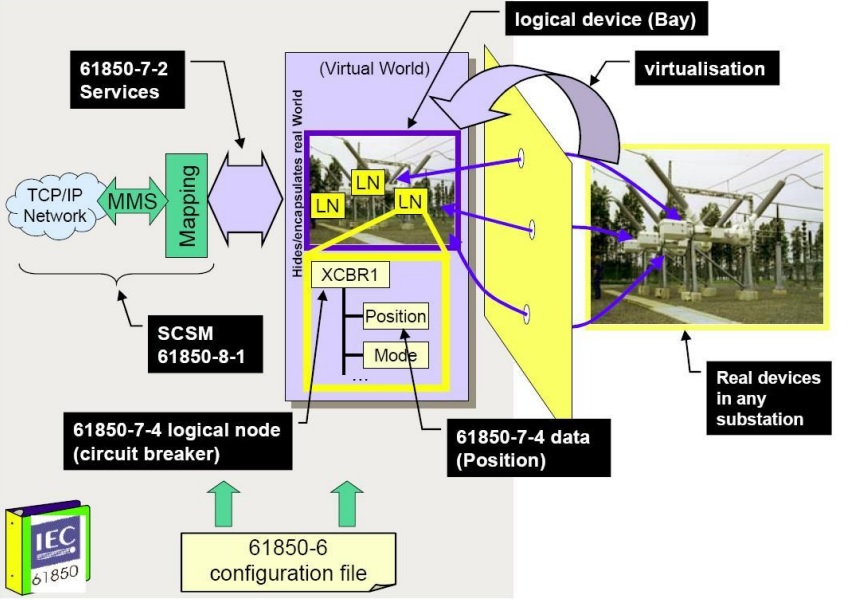
\includegraphics[scale=0.45]{img/IEC61850-model-approach.jpg}
    \caption{Pristup modeliranju trafostanice\footnotemark}
    \label{fig:iec-model-approach}
\end{figure}
\footnotetext{Preuzeto sa \citep{zhang2007iec}}

\begin{figure}[tph]
    \centering
    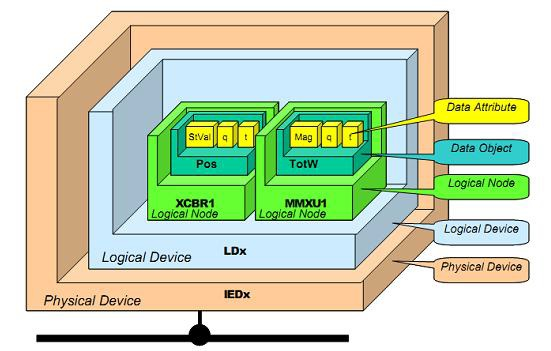
\includegraphics[scale=0.75]{img/IEC61850-physical-device.jpg}
    \caption{Fizički uređaj\footnotemark}
    \label{fig:iec-physical-device}
\end{figure}
\footnotetext{Preuzeto sa \citep{typhoon:MMS}}

Svaki logički uređaj sadrži jedan ili više logičkih čvorova \engl{logical node, LN}. Logički čvor predstavlja skup podataka i prikladnih servisa koji su međusobno logički povezani s jednom zajedničkom funkcijom elektroenergetskog sustava.

Na slici \ref{fig:iec-logical-node-xcbr} se vidi primjer logičkog čvora koji predstavlja prekidač (XCBR). On se sastoji od jednog ili više podatkovnih polja s jedinstvenim imenima. Podatkovna polja \textit{Pos}, koje predstavlja položaj prekidača, i \textit{BlkOpn}, koji predstavlja blok naredbi kad je prekidač u otvorenom položaju. Osim navedenih polja, \textit{XCBR} logički čvor ima još podatkovnih polja koja nećemo razmatrati. Svako podatkovno polje je usklađeno s CDC specifikacijom. Svaki CDC razred opisuje tip i strukturu podataka u logičkom čvoru. Sa slike \ref{fig:iec-logical-node-xcbr} vidimo da se podatkovno polje \textit{Pos} sastoji od niza podatkovnih atributa vezanih za upravljanje, status, supstituciju i konfiguraciju \citep{baigent2004iec}.

\bigskip
Imenovanje logičkih čvorova je standardizirano je u sedmom poglavlju IEC 61850 standarda. Svaka klasa imena logičkog čvora povezana je s nekom funkcijom elektroenergetskog sustava. Osim imena klase, logički čvor u postfiksu ima svoj broj instance. Također može imati opcionalni prefiks koji se odnosi na njegovu ulogu u uređaju. Na slici \ref{fig:iec-logical-node-name} možete vidjeti primjer imenovanja prekidača. Prvo slovo u imenu klase logičkog čvora također određuje njegovu ulogu:

\begin{itemize}
    \item "A" za automatsko upravljanje
    \item "C" za nadzornu kontrolu
    \item "G" za generičke funkcije
    \item "I" za sučelje/arhiviranje
    \item "L" za logički čvor sustava
    \item "M" za mjerenje
    \item "P" za zaštitu
    \item "R" za logičke čvorove vezane za zaštitu
    \item "S" za senzore
    \item "T" za mjerni transformator
    \item "X" za sklopni uređaj
    \item "Y" za energetski transformator
    \item "Z" za ostalo
\end{itemize}

Kako bi bilo moguće referencirati svaki podatkovni atribut unutar IED uređaja osmišljeno je jendoznačno pravilo kod imenovanja IED objekata prikazano na slici \ref{fig:iec-object-name} \citep{baigent2004iec}.

\begin{figure}[tph]
    \centering
    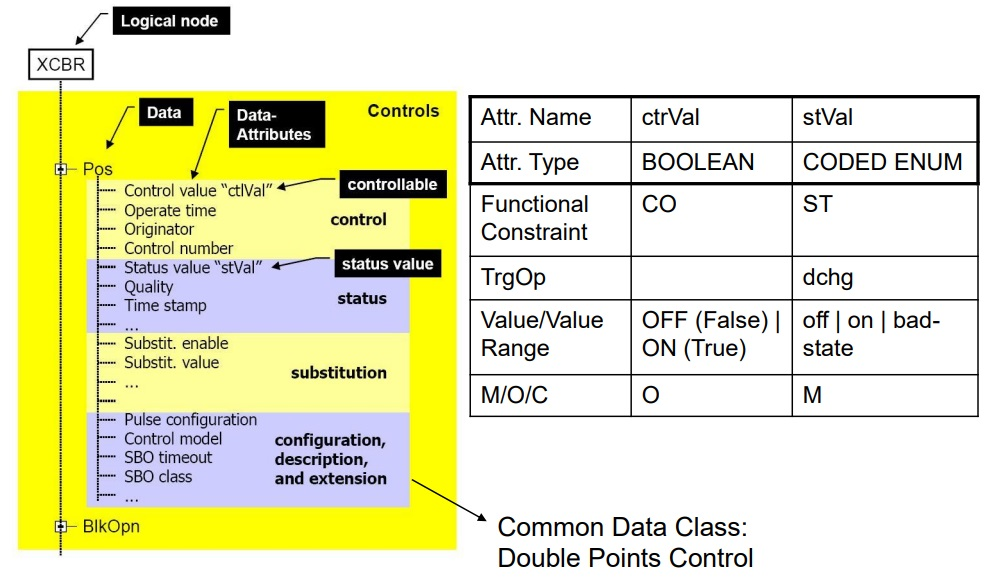
\includegraphics[scale=0.4]{img/IEC61850-logical-node-xcbr.jpg}
    \caption{Primjer logičkog čvora\footnotemark}
    \label{fig:iec-logical-node-xcbr}
\end{figure}
\footnotetext{Preuzeto sa \citep{zhang2007iec}}

\begin{figure}[tph]
    \centering
    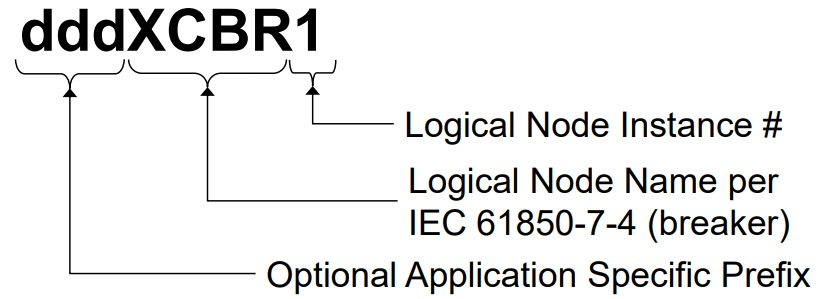
\includegraphics[scale=0.35]{img/IEC61850-logical-node-name.jpg}
    \caption{Imenovanje logičkog čvora\footnotemark}
    \label{fig:iec-logical-node-name}
\end{figure}
\footnotetext{Preuzeto sa \citep{zhang2007iec}}

\begin{figure}[bph]
    \centering
    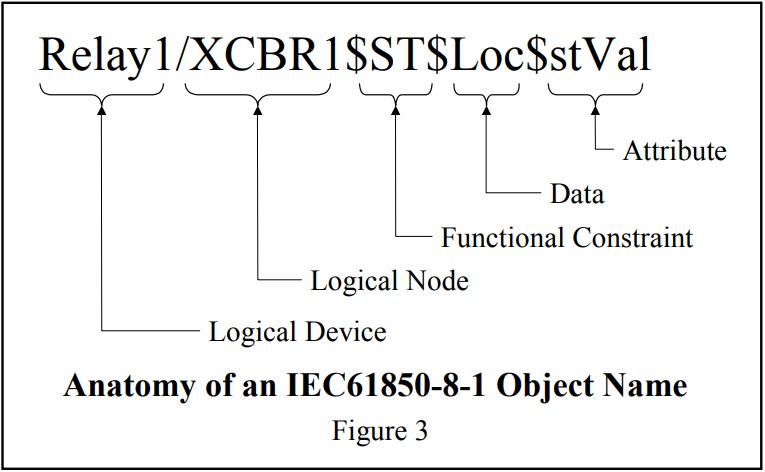
\includegraphics[scale=0.35]{img/IEC61850-object-name.jpg}
    \caption{Imenovanje IED objekta\footnotemark}
    \label{fig:iec-object-name}
\end{figure}
\footnotetext{Preuzeto sa \citep{baigent2004iec}}

\section{Skupovi podataka}
IEC 61850 omogućuje grupiranje podataka logičkih čvorova u skupove podataka (engl. \textit{Data Sets}). Standard IEC 61850 definira pet ACSI usluga povezanih sa skupovima podataka:
\begin{itemize}
    \item \textit{GetDataSetValues} za dobivanje vrijednosti svih članova skupa podataka
    \item \textit{SetDataSetValues} za postavljanje vrijednosti svih članova skupa podataka
    \item \textit{CreateDataSet} za dinamičko stvaranje novog skupa podataka
    \item \textit{DeleteDataSet} za brisanje skupa podataka koji je stvoren
    \item \textit{GetDataSetDirectory} za dobivanje popisa svih postojećih skupova podataka na poslužitelju
\end{itemize}

\bigskip
Skupovi podataka mogu se koristiti za čitanje ili pisanje nekoliko podatkovnih objekata ili podatkovnih atributa odjednom korištenjem \textit{GetDataSetValues} i \textit{SetDataSetValues} ACSI usluga. Koncept skupa podataka također koriste usluge izvješćivanja, zapisivanja, MMS, GOOSE i SV. Postoje dvije vrste skupova podataka.

\subsection{Perzistentni skupovi podataka}
Imaju referencu u formau \textit{LDName/LNName.} \textit{DataSetName}. Vidljivi su svim klijentima. Perzistentni skupovi podataka mogu se unaprijed konfigurirati u SCL datoteci. Perzistentni skupovi podataka definirani u SCL datoteci se ne mogu izbrisati. Klijenti mogu dinamički kreirati perzistentne skupove podataka te se takvi skupovi podataka kasnije mogu ponovo izbrisati. Dinamički stvoreni skupovi podataka automatski se brišu nakon što se poslužitelj zaustavi.

\subsection{Neperzistentni skupovi podataka}
Imaju referencu u formatu \textit{@datasetname}. Vidljivi su samo klijentu koji ih je stvorio putem ACSI usluge \textit{CreateDataSet}. Ovakvi skupovi podataka postoje samo dok je veza otvorena.

\section{Izvještavanje}
Izvještavanje omogućuje poslužitelju slanje podataka na temelju događaja bez izričitog zahtjeva klijenta. Podaci koji se šalju i događaji koji uzrokuju izvješća konfiguriraju se putem kontrolnih blokova za izvješćivanje \engl{Report Control Block, RCB}. Standard razlikuje dvije vrste izvješćivanja:
\begin{itemize}
    \item izvješćivanje s međuspremnikom
    \item izvješćivanje bez međuspremnika
\end{itemize}
Kod izvješćivanja s međuspremnikom poslužitelj sprema izvješća u međuspremnik u slučaju prekida veze s klijentom. Na ovaj način izvješća se mogu poslati nakon što se klijent ponovno spoji. Izvještavanje s međuspremnikom konfigurira se putem kontrolnih blokova za izvješćivanje s međuspremnikom \engl{Buffered Report Control Blocks, BRCB}. Izvješćivanje bez međuspremnika konfigurira se putem kontrolnih blokova za izvješćivanje bez međuspremnika \engl{Unbuffered Report Control Blocks, URCB}.

\subsection{RCB blokovi}
RCB blokovi se nalaze unutar logičkih čvorova podatkovnog modela poslužitelja te su definirani u SCL konfiguracijskim datotekama. Oni su fiksni i ne mogu se brisati ili dodavati tijekom izvođenja. Na RCB blok se može pretplatiti samo jedan klijent, nije moguće posluživati više klijenata paralelno. RCB blokovi su uvijek povezani s određenim skupom podataka. Iako RCB blokovi mogu referencirati samo skupove podataka koji se nalaze u istom logičkom čvoru kao i sam RCB blok, oni i dalje mogu nadzirati podatke iz drugih logičkih čvorova jer se članovi skupa podataka mogu nalaziti u drugim logičkim čvorovima. Klijent može dinamički mijenjati pridruženi skup podataka RCB bloka tijekom izvođenja. Pošto se RCB blokovi nalaze u logičkim čvorovima, njihove reference su formata \textit{LDName/LNName.RCBName}. RCB blokovi šalju izvješća o pridruženim skupovima podataka svojim klijentima kada se dogodi neki od događaja definiranih za taj RCB blok u SCL konfiguracijskoj datoteci. Sljedeći događaji mogu uzrokovati da RCB blok pošalje izvješće \citep{beanit:data-sets}:
\begin{itemize}
    \item Klijent zatraži opće izvješće \engl{general interrogation}
    \item Promjena nekog od elemenata skupa podataka pridruženog RCB bloku
    \item Omogućeno je slanje povremenih izvješća u konfiguraciji RCB bloka
\end{itemize}

\chapter{Komunikacija}
Sučelje apstraktnih komunikacijskih usluga \engl{Abstract Communication Service Interface, ACSI} prema IEC 61850 standardu definira skup usluga i odgovora na te usluge koji omogućuje svim IED uređajima da na identičan način prenose podatke preko mreže. Vremenski osjetljive poruke se preslikavaju na GOOSE i SV protokol, a vremenski neosjetljive poruke na MMS protokol \citep{baigent2004iec}.

\section{MMS protokol}
MMS protokol \engl{Manufacturing Message Specification, MMS} je poslužitelj/kli\-jent oblik komunikacije. Ovaj protokol služi za razmjenu informacije između IED uređaja te za komunikaciju IED uređaja s uređajima više razine poput računalnih sustava za nadzor, mjerenje i upravljanje \engl{Supervisory Control and Data Acquisition, SCADA}. Primjer takve komunikacije vidi se na slici \ref{fig:iec-mms}. Jedinica za udaljen pristup \engl{Remote Termunal Unit, RTU} služi za povezivanje IED uređaja i SCADA sustava. Ispod MMS protokola nalaze se TCP/IP protokoli te se time omogućuje pristup MMS poslužiteljima putem IP adrese. Klijenti MMS protokola mogu čitati/pisati podatke, čitati konfiguraciju i razmjenjivati datoteke. Jedna od uloga MMS protokola je automatsko dojavljivanje promjena u skupovima podataka klijentima bez da klijenti zatraže čitanje podataka, a to se ostvaruje pomoću RCB blokova \citep{typhoon:MMS}. Preslikavanje ACSI sučelja na MMS možemo vidjeti u tablicama \ref{tab:iec-to-mms-objects} i \ref{tab:iec-to-mms-services}.

\begin{figure}[tph]
    \centering
    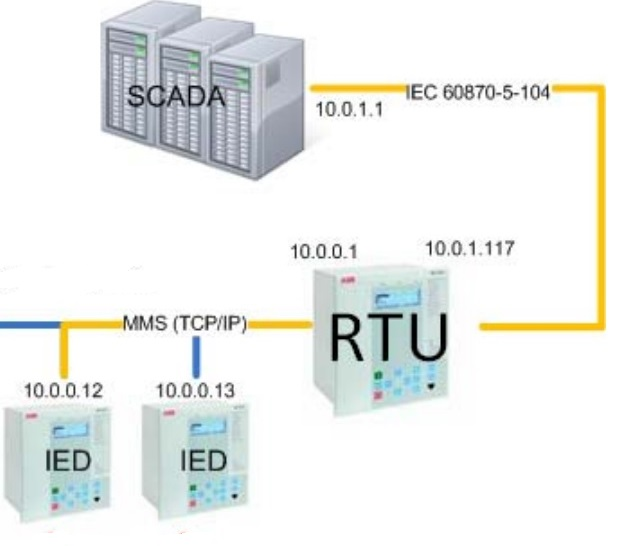
\includegraphics[scale=0.6]{img/IEC61850-MMS.jpg}
    \caption{Komunikacija putem MMS protokola\footnotemark}
    \label{fig:iec-mms}
\end{figure}
\footnotetext{Preuzeto s \citep{honeth:IEC}}

\begin{table}[tph]
    \centering
    \begin{tabular}{ |l|l| }
        \hline
        \multicolumn{1}{|c|}{\textbf{IEC 61850 Objekti}} &
        \multicolumn{1}{|c|}{\textbf{MMS Objekt}} \\
        \hline \hline
        SERVER class & Virtual Manufacturing Device \\
        \hline
        LOGICAL DEVICE class & Domain \\
        \hline
        LOGICAL NODE class & Named Variable \\
        \hline
        DATA class & Named Variable \\
        \hline
        DATA-SET class & Named Variable List \\
        \hline
        SETTING-GROUP-CONTROL-BLOCK & Named Variable \\
        class & \\
        \hline
        REPORT-CONTROL-BLOCK class  & Named Variable \\
        \hline
        LOG class & Journal \\
        \hline
        LOG-CONTROL-BLOCK class & Named Variable \\
        \hline
        GOOSE-CONTROL-BLOCK class & Named Variable \\
        \hline
        GSSE-CONTROL-BLOCK class & Named Variable \\
        \hline
        CONTROL class & Named Variable \\
        \hline
        Files & Files \\
        \hline
    \end{tabular}
    \caption{Preslikavanje IEC 61850 objekata na MMS objekte\footnotemark}
    \label{tab:iec-to-mms-objects}
\end{table}
\footnotetext{Preuzeto s \citep{baigent2004iec}}

\begin{table}[tph]
    \centering
    \begin{tabular}{ |l|l| }
        \hline
        \multicolumn{1}{|c|}{\textbf{IEC 61850 Usluge}} &
        \multicolumn{1}{|c|}{\textbf{MMS Usluge}} \\
        \hline \hline
        LogicalDeviceDirectory & GetNameList \\
        \hline
        GetAllDataValues & Read \\
        \hline
        GetDataValues & Read \\
        \hline
        SetDataValues & Write \\
        \hline
        GetDataDirectory & GetNameList \\
        \hline
        GetDataDefinition & GetVariableAccessAttributes \\
        \hline
        GetDataSetValues & Read \\
        \hline
        SetDataSetValues & Write \\
        \hline
        CreateDataSet & CreateNamedVariableList \\
        \hline
        DeleteDataSet & DeleteNamedVariableList \\
        \hline
        GetDataSetDirectory & GetNameList \\
        \hline
        Report (Buffered and Unbuffered) & InformationReport \\
        \hline
        GetBRCBValues/GetURCBValues & Read \\
        \hline
        SetBRCBValues/SetURCBValues & Write \\
        \hline
        GetLCBValues & Read \\
        \hline
        SetLCBValues & Write \\
        \hline
        QueryLogByTime & ReadJournal \\
        \hline
        QueryLogAfter & ReadJournal \\
        \hline
        GetLogStatusValues & GetJournalStatus \\
        \hline
        Select & Read/Write \\
        \hline
        SelectWithValue & Read/Write \\
        \hline
        Cancel & Write \\
        \hline
        Operate & Write \\
        \hline
        Command-Termination & Write \\
        \hline
        TimeActivated-Operate & Write \\
        \hline
        GetFile & FileOpen/FileRead/FileClose \\
        \hline
        SetFile & ObtainFile \\
        \hline
        DeleteFile & FileDelete \\
        \hline
        GetFileAttributeValues & FileDirectory \\
        \hline
    \end{tabular}
    \caption{Preslikavanje IEC 61850 usluga na MMS usluge\footnotemark}
    \label{tab:iec-to-mms-services}
\end{table}
\footnotetext{Preuzeto s \citep{baigent2004iec}}

\clearpage

\section{GOOSE protokol}
GOOSE protokol \engl{Generic Object Oriented Substation Event} je izdavač/pret\-pla\-tnik oblik komunikacije. Ovaj protokol se također koristi za komunikaciju između IED uređaja (slika \ref{fig:iec-goose-simple}), ali za razliku od MMS protokola, GOOSE protokol se direktno preslikava na \textit{Ethernet} okvir. Time se eliminira obrada bilo kakvih srednjih slojeva i osigurava da se vremenski osjetljive poruke dostave na vrijeme.

\begin{figure}[tph]
    \centering
    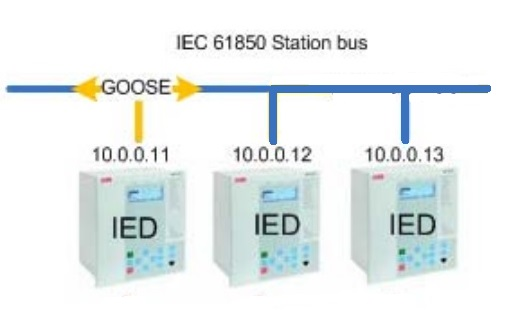
\includegraphics[scale=0.6]{img/IEC61850-GOOSE-simple.jpg}
    \caption{Komunikacija između IED uređaja putem GOOSE protokola\footnotemark}
    \label{fig:iec-goose-simple}
\end{figure}
\footnotetext{Preuzeto sa \citep{honeth:IEC}}

GOOSE protokol se temelji na obradi događaja koristeći RCB blokove. Koncept GOOSE komunikacije je da izdavač povremeno šalje kontrolne poruke, a kada se dogodi neki događaj, izdavač šalje niz identičnih poruka s novim podatcima. Slanjem niza identičnih poruka smanjuje se mogućnost gubitka poruke s obzirom na to da protokol nema mehanizam kojim bi pretplatnik potvrdio da je primio poruku. Sve poruke se objavljuju pod temom. Pretplatnik prima sve poruke iz sustava, ali filtrira i analizira samo poruke poslane unutar pretplaćene teme. Komunikacija pomoću GOOSE protokola moguća je samo unutar lokalne (LAN) mreže \citep{typhoon:GOOSE}.

Na slici \ref{fig:iec-goose-complex} vidimo primjer komunikacije između izdavača i pretplatnika korištenjem GOOSE protokola. U prvom dijelu komunikacije vidimo da pretplatnik dohvaća podatke od izdavača preko \textit{GetDataValue} ACSI usluge. U drugom dijelu komunikacije vidimo da se jednom od elemenata podatkovnog skupa promijenila vrijednost zbog čega izdavač šalje informaciju o promjeni svim svojim pretplatnicima pomoću \textit{Publish} ACSI usluge. Također je važno primijetiti da se izvješća drže u međuspremniku što nas upućuje na to da je korišten BRCB blok. Na kraju pretplatnik šalje \textit{Generic Substation State Event (GSSE)} poruku. GSSE protokol je nešto jednostavnija verzija GOOSE protokola preslikana na IEC/ISO 8802-2 i 8802-3. Namijenjen je za zastarjele uređaje i unazadnu kompatibilnost te ga nećemo dalje razmatrati \citep{wiki:GSSE}.

\begin{figure}[tph]
    \centering
    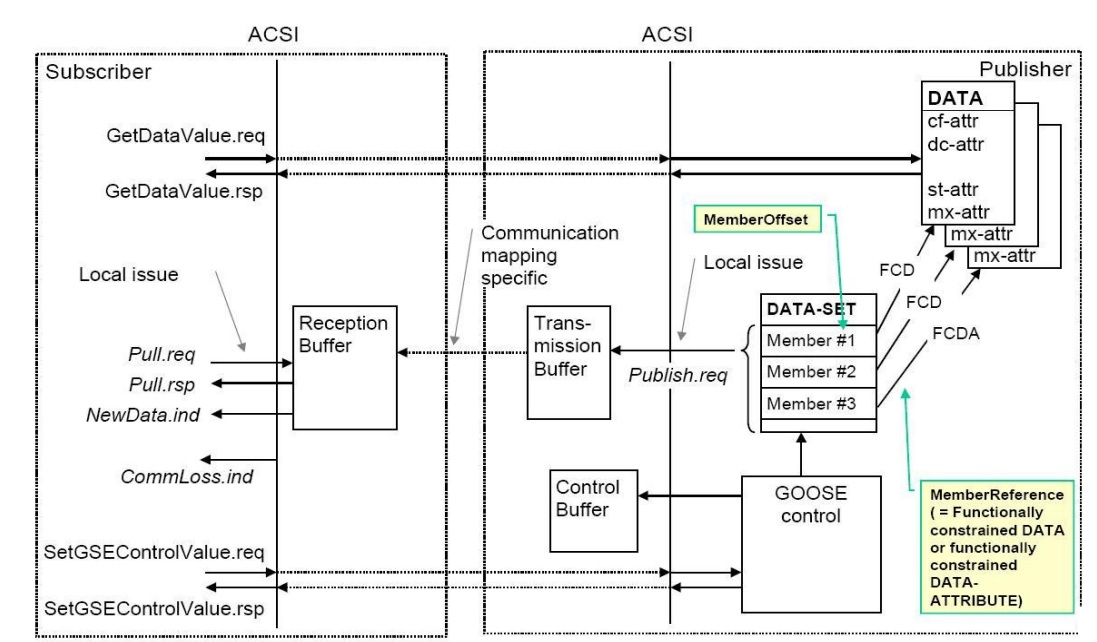
\includegraphics[scale=0.5]{img/IEC61850-GOOSE-complex.jpg}
    \caption{Komunikacija između GOOSE izdavača i pretplatnika\footnotemark}
    \label{fig:iec-goose-complex}
\end{figure}
\footnotetext{Preuzeto sa \citep{zhang2007iec}}

\section{SV protokol}
Da bismo razumjeli ulogu SV protokola prvo se moramo upoznati s procesnom sabirnicom \engl{Process Bus}.

\subsection{Procesna sabirnica}
Procesni sloj dodan je u model trafostanice kako bi se omogućilo prikupljanje podataka o naponu, struji i statusu transformatora i pretvarača u digitalnom obliku. Svi podatci o naponu, struju i statusu šalju se u sabirne jedinice \engl{Merge Unit, MU}. MU jedinice uzorkuju podatke dogovorenom i sinkroniziranom brzinom. Tako svaki IED uređaj može usklađeno primati podatke od više MU jedinica. Trenutno su definirane dvije frekvencije uzorkovanja:
\begin{itemize}
    \item 80 uzoraka po ciklusu za osnovnu zaštitu i nadzor
    \item 256 uzoraka po ciklusu za visokofrekventne primjere
\end{itemize}
Duljina ciklusa ovisi o frekvenciji mjerenog signala. Uzmimo za primjer frekvenciju mjerenog signala od 50 Hz i frekvenciju uzorkovanja 80 uzoraka po ciklusu. Tada bi period uzorkovanja bio:
\[
T\textsubscript{uzorkovanja} = \frac{1}{50 Hz \cdot 80} = 250 \mu s
\]

IEC 61850 definira prenošenje ovih podataka putem dvije različite definicije protokola. Poglavlje 9.1 definira \textit{Unidirectional Multidrop Point-to-Point} fiksnu vezu koja prenosi fiksni skup podataka i nećemo je dalje razmatrati. Poglavlje 9.2 definira konfigurabilni skup podataka koji se prenosi višestruko od jednog izdavača na više pretplatnika. U definiciju iz poglavlja 9.2 upada SV protokol. Oba poglavlja definiraju da se protokoli preslikavaju direktno u \textit{Ethernet} okvire kako bi se izbjegla obrada srednjih slojeva. Ovisno o brzini uzorkovanja, na jedan 100MB \textit{Ethernet} priključak može se povezati od 1 do 5 MU jedinica. Više 100MB \textit{Ethernet} priključaka može se zatim kombinirati u jedan \textit{Ethernet} preklopnik s okosnicom od 1GB. U ovoj konfiguraciji moguće je dostavljati i do 50 skupova podataka pretplatnicima \citep{baigent2004iec}.

\subsection{Protokol uzorkovanih vrijednosti}
Protokol uzorkovanih vrijednosti \engl{Sampled Values, SV} je oblik komunikacije izdavač/pretplatnik. Ovaj protokol se koristi za razmjenu informacija između MU jedinica i IED uređaja preko \textit{Etherneta}. Na slici \ref{fig:iec-process-bus-sv} ja prikazana komunikacija MU jedinice i IED uređaja putem procesne sabirnice koristeći SV protokol. Kao i kod GOOSE protokola, sve poruke se objavljuju pod temom. Pretplatnik prima sve poruke iz sustava, ali filtrira i analizira samo poruke poslane s pretplaćenom temom. Ovaj protokol moguće je koristiti samo unutar lokalne (LAN) mreže \citep{typhoon:SV}.

\begin{figure}[tph]
    \centering
    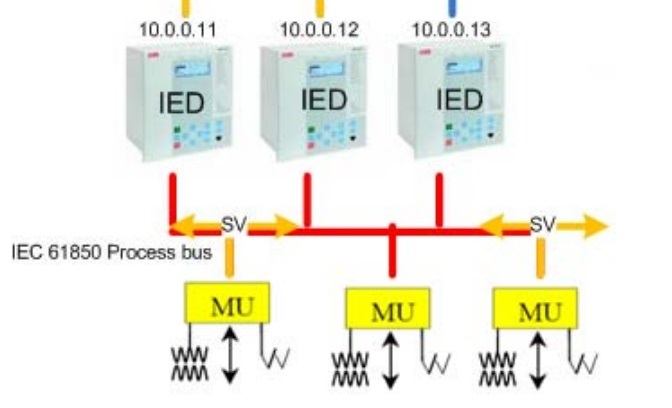
\includegraphics[scale=0.6]{img/IEC61850-process-bus-sv.jpg}
    \caption{Komunikacija preko procesne sabirnice\footnotemark}
    \label{fig:iec-process-bus-sv}
\end{figure}
\footnotetext{Preuzeto sa \citep{honeth:IEC}}

\section{Šira slika}
Na slici \ref{fig:iec-architecture} se vidi pojednostavljena arhitektura komunikacijskog sustava IEC 61850 trafostanice. Na procesnom sloju podaci iz optičkih/elektroničkih senzora napona, struje i informacije o statusu  prikupljaju se i digitaliziraju u MU jedinicama. MU jedinice se mogu fizički nalaziti na terenu ili u kontrolnoj kući. Podaci iz MU jedinica će se prikupljati preko redundantnih 100MB optičkih \textit{Ethernet} veza. Te \textit{Ethernet} veze zatim se kombiniraju u redundantne  \textit{Ethernet} preklopnike s  okosnicom od 1GB koji podržavaju prioritetni \textit{Ethernet} i \textit{Ethernet Virtual LAN} (VLAN). VLAN omogućuje \textit{Ethernet} preklopniku isporuku skupova podataka samo onim priključcima/IED uređajima koji su pretplaćeni za primanje podataka. Komunikacija na ovoj razini se odvija uz pomoć SV protokola.

\begin{figure}[tph]
    \centering
    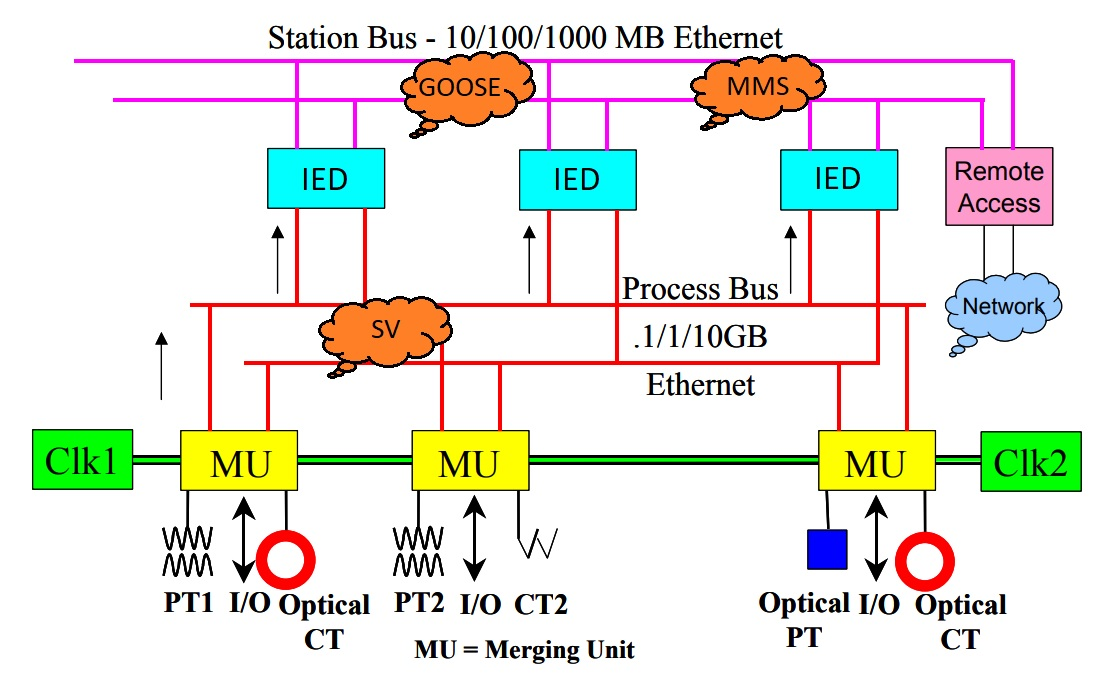
\includegraphics[scale=0.4]{img/IEC61850-architecture.jpg}
    \caption{Arhitektura komunikacijskog sustava IEC 61850 trafostanice\footnotemark}
    \label{fig:iec-architecture}
\end{figure}
\footnotetext{Preuzeto sa \citep{honeth:IEC}}

Također je potrebno obratiti pažnju na redundantne sinkronizacijske satove. U ovoj arhitekturi, ako dođe do kvara prvog sinkronizacijskog sata, drugi sinkronizacijski sat će se automatski uključiti i nastaviti pružati sinkronizaciju uzorkovanja.

Na razini trafostanice postoji sabirnica \engl{Station Bus} koja se temelji na 10MB i 100MB \textit{Ethernetu}. Ona osigurava primarnu komunikaciju između različitih logičkih čvorova IED uređaja koji pružaju različite funkcije zaštite, kontrole i nadzora stanice. Komunikacija na ovoj razini se odvija pomoću GOOSE i MMS protokola. Na ovoj razini je također poželjno imati redundantnu komunikacijsku arhitekturu jer u slučaju kvara i prekida komunikacijskih veza između IED uređaja može doći do ozbiljnijih oštećenja na trafostanici.

Konačno, ova arhitektura podržava udaljeni pristup mreži za sve vrste čitanja i pisanja podataka. Udaljeni klijenti imaju pristup širokom spektru dostupnih informacija. Tipični klijenti su:
\begin{itemize}
    \item lokalna sučelja \engl{Human Machine Interface, HMI}
    \item operateri
    \item inženjeri
    \item tim za održavanje
\end{itemize}

Kod udaljene pristupne točke potrebno je implementirati sigurnosne funkcije kao što su enkripcija i autentifikacija. Ovakva implementacija rasterećuje pojedinačne IED uređaje od izvođenja enkripcije na internim prijenosima podataka, ali i dalje pruža sigurnost na svim vanjskim transakcijama \citep{baigent2004iec}.

\chapter{SCL jezik}
Jezik za konfiguraciju trafostanica \engl{Substation Configuration Language, SCL} se temelji na \textit{eXtensible Markup Language} (XML) jeziku te služi za opisivanje sustava temeljenih na IEC 61850 standardu. SCL specificira hijerarhiju jednoznačnih i standardiziranih XML konfiguracijskih datoteka koje omogućuju konfiguriranje trafostanice na više razina \citep{baigent2004iec}. SCL datoteke se razmjenjuju između različitih konfiguratora i IED uređaja tijekom procesa konfiguracije. Sudionici u procesu konfiguracije trafostanice su:
\begin{itemize}
    \item konfigurator IED uređaja
    \item konfigurator sustava
    \item IED uređaj
\end{itemize}

\section{Vrste SCL datoteka}
IED 61850 definira šest različitih SCL datoteka te svaka od njih ima zasebnu ulogu u konfiguriranju trafostanice. Svaka datoteka sadrži broj verzije i broj revizije kako bi se razlikovale revidirane i stare datoteke \citep{aftab2019novel}.

\subsection{IED Capability Description (ICD) datoteka}
Ova datoteka sadrži pregled funkcionalnosti i mogućnosti IED uređaja u obliku predloška kojeg proizvođač  isporučuje zajedno s IED uređajem. Vlasnik može izmjenjivati taj predložak kako bi implementirao dodatne mogućnosti. ICD datoteka također sadrži logičke čvorove i odgovarajuće tipove podataka povezane s mogućnostima IED uređaja. ICD datoteku IED konfigurator šalje konfiguratoru sustava nakon svake izmjene rasporeda sustava, tj. u slučaju dodavanja ili uklanjanja IED uređaja u sustavu, kako bi se trafostanica ponovno konfigurirala. Ekstenzija datoteke koja se koristi za ICD datoteku je \textit{.icd}.

\subsection{Instantiated IED Description (IID) datoteka}
Ova datoteka sadrži instancirane podatkovne objekte dobivene iz predloška podataka i koristi se kada je potrebno izvršiti određene izmjene u IED uređaju. Budući da se proces konfiguracije IED uređaja odvija višestrukim razmjenama konfiguracijskih datoteka, izmjena mogućnosti IED uređaja u kasnijoj fazi može se izvršiti putem IID datoteke. Obično je potrebno uključiti unaprijed konfiguriranu datoteku instance za IED uređaj, u slučaju da se vrijednost instance promijeni ili dođe do drugih manjih izmjena. Ekstenzija datoteke koja se koristi za razlikovanje ove vrste datoteke je \textit{.iid}.

\subsection{System Specification Description (SSD) datoteka}
Ova datoteka se šalje iz alata za specifikaciju sustava u konfigurator sustava. Sadrži pregled strukture trafostanice kao dijagram s jednom linijom, funkcije trafostanice i potrebne logičke čvorove. Također sadrži predloške tipova  podataka za pridružene logičke čvorove. Ekstenzija datoteke koja se koristi za ovu datoteku je \textit{.ssd}.

\subsection{System Configuration Description (SCD) datoteka}
Ovu datoteku generira konfigurator sustava nakon kombiniranja svih ICD datoteka dobivenih iz različitih IED konfiguratora. Ova datoteka sadrži potpuni opis procesa uključujući konfiguraciju za sve IED uređaje prisutne u trafostanici, strukturu ili izgled trafostanice i konfiguraciju komunikacije. Ekstenzija datoteke koja se koristi za SCD datoteku je \textit{.scd}.

\subsection{Configured IED Description (CID) datoteka}
Ova datoteka sadrži sve informacije potrebne za odgovarajući IED uređaj. Ona opisuju instancirani IED uređaj unutar projekta. Sadrži potpuni opis IED uređaja i njegovu adresu. CID datoteka se dijeli sa svim drugim IED uređajima prije početka rada sustava. Konfigurator sustava vraća ovu datoteku IED konfiguratoru nakon završetka procesa konfiguracije. Ekstenzija datoteke koja se koristi za CID datoteku je \textit{.cid}.

\subsection{System Exchange Description (SED) datoteka}
Ova datoteka služi za konfiguriranje komunikacije između dvije trafostanice u IEC 61850 komunikacijskoj mreži. Ekstenzija datoteke koja se koristi za SED datoteku je \textit{.sed}.

\section{Proces generiranja konfiguracijskih datoteka}
U procesu generiranja konfiguracijskih datoteka konačni cilj je SCD datoteka. Ona sadrži informacije o svim IED uređajima, rasporedu trafostanice, tipovima podataka i pridruženim logičkim čvorovima te opis komunikacije. Na slici \ref{fig:iec-scl} je prikazan tijek generiranja različitih vrsta SCL datoteka.

\subsection{Konfiguriranje unutar trafostanice}
Na početku svaki IED uređaj dostavlja svoju ICD datoteku IED konfiguratoru. U slučaju da je potrebna bilo kakva izmjena u opisu IED uređaja tijekom procesa konfiguracije, IID datoteka se dostavlja u IED konfigurator. IED konfiguratori prikupljaju sve ICD i IID datoteke od različitih IED uređaja te ih zatim šalju konfiguratoru sustava.

\smallskip
Sada konfigurator sustava ima opise mogućnosti svih IED uređaja. Nakon toga se konfiguratoru sustava dostavlja SSD datoteka iz alata za specifikaciju sustava. SSD datoteka sadrži osnovne informacije o izgledu sustava i potrebnim logičkim čvorovima. Konfigurator sustava zatim kombinira sve ove informacije i generira SCD datoteku.

\smallskip
Generirana SCD datoteka konačno se dijeli s IED konfiguratorima, koji pomoću SCD datoteke i ICD datoteka generiraju CID datoteku za svaki IED uređaj. CID datoteka sadrži osnovni pregled konfiguracije sustava zajedno s adresama svih povezanih IED uređaja. Dijeli se sa svim IED uređajima u trafostanici prije početka rada.

\smallskip
Ovaj proces se ponavlja nekoliko puta kako bi se osiguralo da su svi dijelovi sustava ispravno konfigurirani. U slučaju dodavanja ili uklanjanja IED uređaja iz sustava, isti se postupak ponavlja.

\begin{figure}[tph]
    \centering
    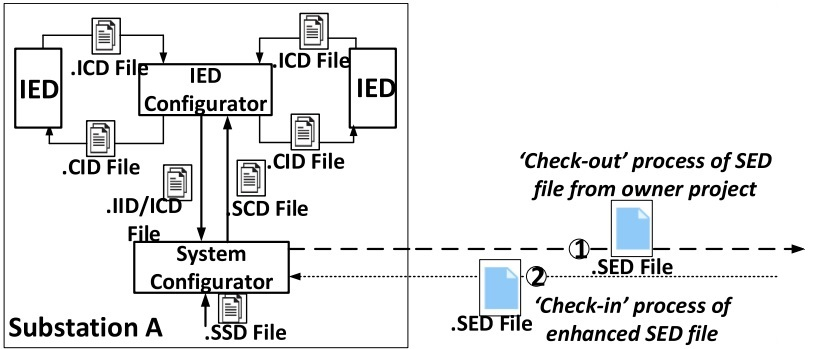
\includegraphics[scale=0.5]{img/IEC61850-SCL.jpg}
    \caption{Postupak generiranja SCL datoteka\footnotemark}
    \label{fig:iec-scl}
\end{figure}
\footnotetext{Preuzeto sa \citep{aftab2019novel}}

\subsection{Konfiguriranje dviju trafostanica}
Postoje i situacije u kojima dvije trafostanice moraju međusobno komunicirati. Jedan takav primjer je zaštita vodova koja zahtjeva da IED uređaj jedne trafostanice zna svojstva IED uređaja druge trafostanice. Ovo je potrebno kako bi se u skup podataka RCB bloka jedne trafostanice dodali podatci iz IED uređaja udaljene trafostanice. Postupak konfiguracije između dvije trafostanice se postiže razmjenom SED datoteka.

\smallskip
Konfigurator sustava lokalne trafostanice \textit{odjavljuje} \engl{Check-out} svoju SED datoteke iz projekta te je šalje udaljenoj trafostanici. Zatražene informacije konfigurator sustava udaljene trafostanice dodaje u SED datoteku koja se zatim vraća lokalnoj trafostanici. Konfigurator sustava lokalne trafostanice nakon toga \textit{prijavljuje} \engl{Check-in} modificiranu vraćenu SED datoteka vlasnički projekt. Time je razmjena podataka obavljena \citep{aftab2019novel}.

\chapter{Rezultati}
Programska implementacija vizualizatora SCL konfiguracijskih datoteka ostvarena je u obliku Web aplikacije. Web aplikacija je podijeljena na klijentsku \engl{frontend} i poslužiteljsku \engl{backend} stranu.

\bigskip

Klijentska strana je pisana u programskom jeziku \textit{JavaScript}. Također su korištene biblioteke:
\begin{itemize}
    \item \textit{React} verzije \textit{18.2.0}
    \item \textit{Bootstrap} verzije \textit{5.2.3}
    \item \textit{Material UI} verzije \textit{5.13.1}
\end{itemize}
Uloga klijentske strana je dobivanje unosa od korisnika. Komponenta \textit{TextInput} služi za čuvanje stanja i uređivanje SCL datoteke. Kako ne bismo morali ručno popunjavati \textit{TextInput} komponentu sadržajem SCL datoteke, moguće je učitati čitavu SCL datoteku pomoću \textit{UploadButton} komponente.

Nakon što \textit{TextInput} komponenta ispunjena sadržajem željene SCL datoteke, postupak vizualizacije pokreće se pomoću \textit{ConvertButton} komponente. \textit{ConvertButton} komponenta šalje sadržaj \textit{TextInput} komponente poslužiteljskoj strani na obradu. Klijentska aplikacija zatim od poslužiteljske strane dobije JSON datoteku dogovorenog formata pomoću koje \textit{TextVisualizer} i \textit{TextNode} komponente generiraju vizualizaciju SCL datoteke.

Prikaz sučelja klijentske strane može se vidjeti na slici \ref{fig:scl-interface}

\begin{figure}[tph]
    \centering
    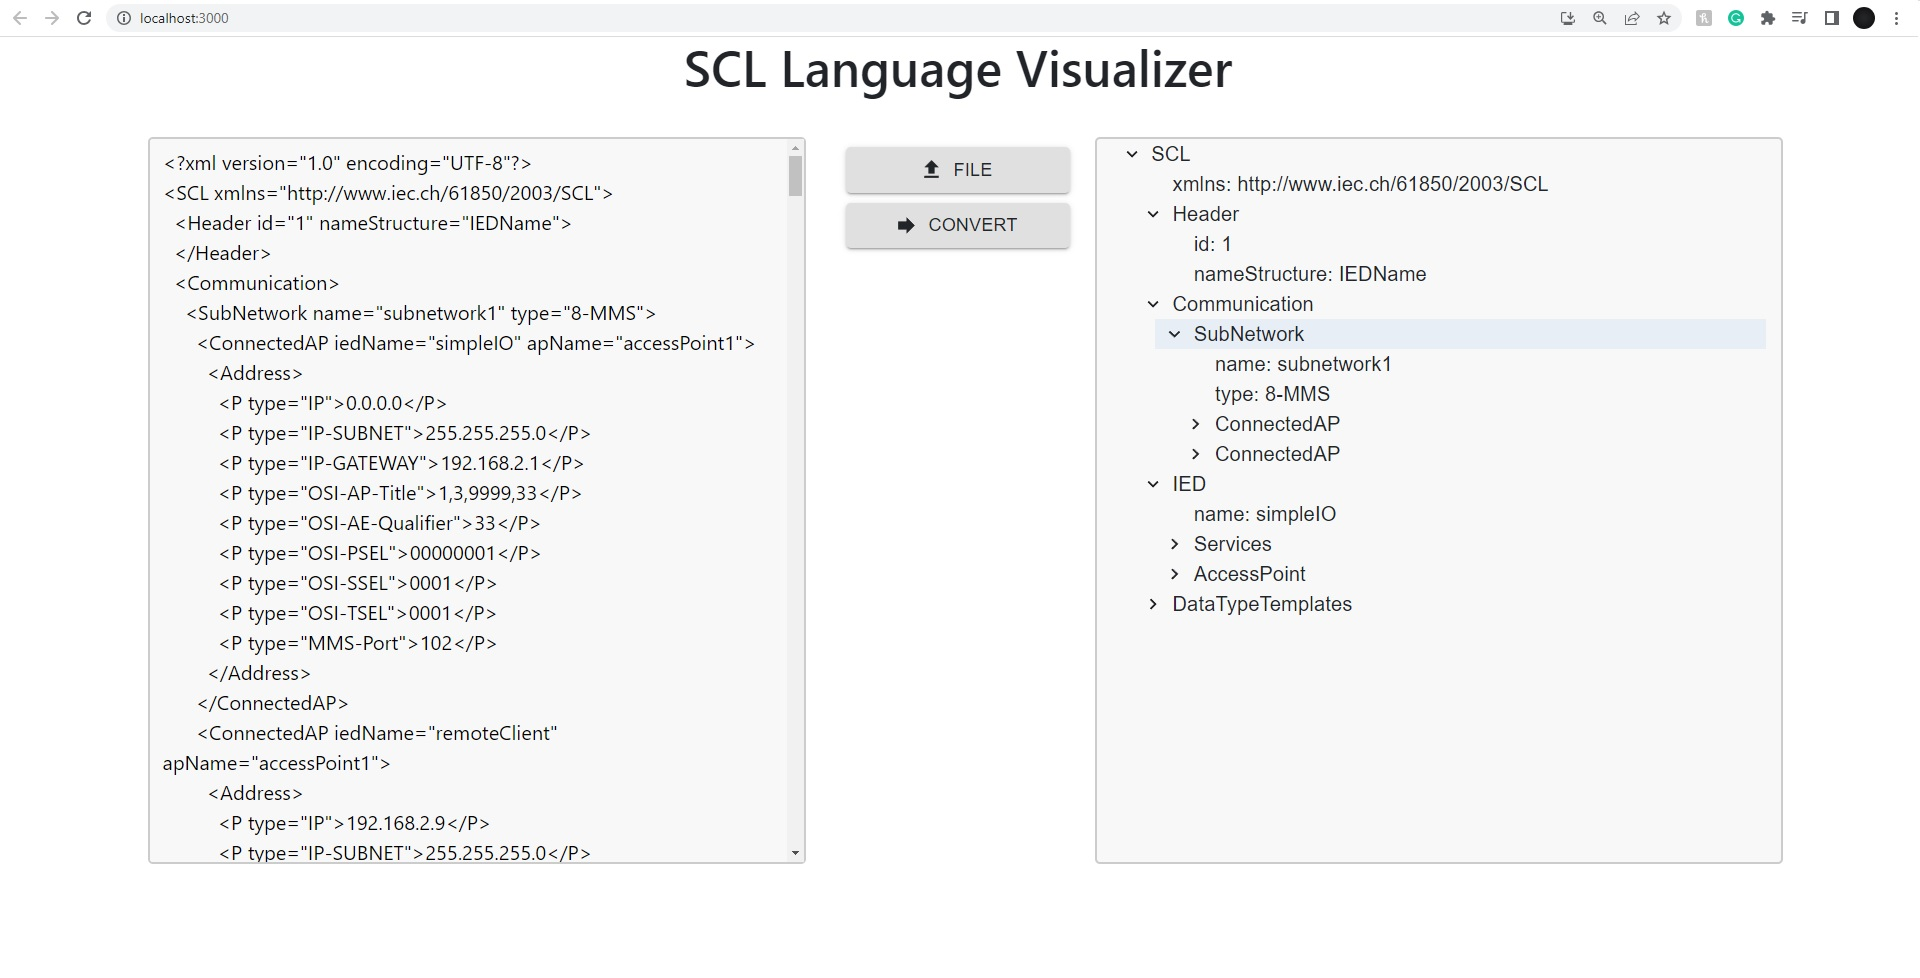
\includegraphics[width=\textwidth]{img/SCL-Visualizer-interface.jpg}
    \caption{Korisničko sučelje klijentske strane}
    \label{fig:scl-interface}
\end{figure}

\bigskip
Poslužiteljska strana je pisana u programskom jeziku \textit{Java} verzije \textit{17}. Također je korišten upravitelj projekta \textit{Maven} verzije \textit{3.8.6} i radni okvir \textit{Spring Boot} verzije \textit{3.0.6}

Uloga poslužiteljske strane je obrada SCL datoteke te generiranje JSON datoteke dogovorenog formata pomoću koju će klijentska strana prikazati vizualizaciju SCL datoteke.

Obrada klijentskog zahtjeva počinje u razredu \textit{SclVisualizerController} koji zahtjev prosljeđuje na \textit{SclParserServiceJpa} razred i vraća klijentu rezultat obrade \textit{SclParserServiceJpa} razreda. \textit{SclParserServiceJpa} razred koristi \textit{SAXParser}, \textit{Javin} nativni XML parser, kako bi generirao JSON datoteku.

U slučaju greške pri obradi, na klijentsku stranu se šalje prikladna poruka koja će se prikazati umjesto vizualizacije (slika \ref{fig:scl-error}).

\begin{figure}[tph]
    \centering
    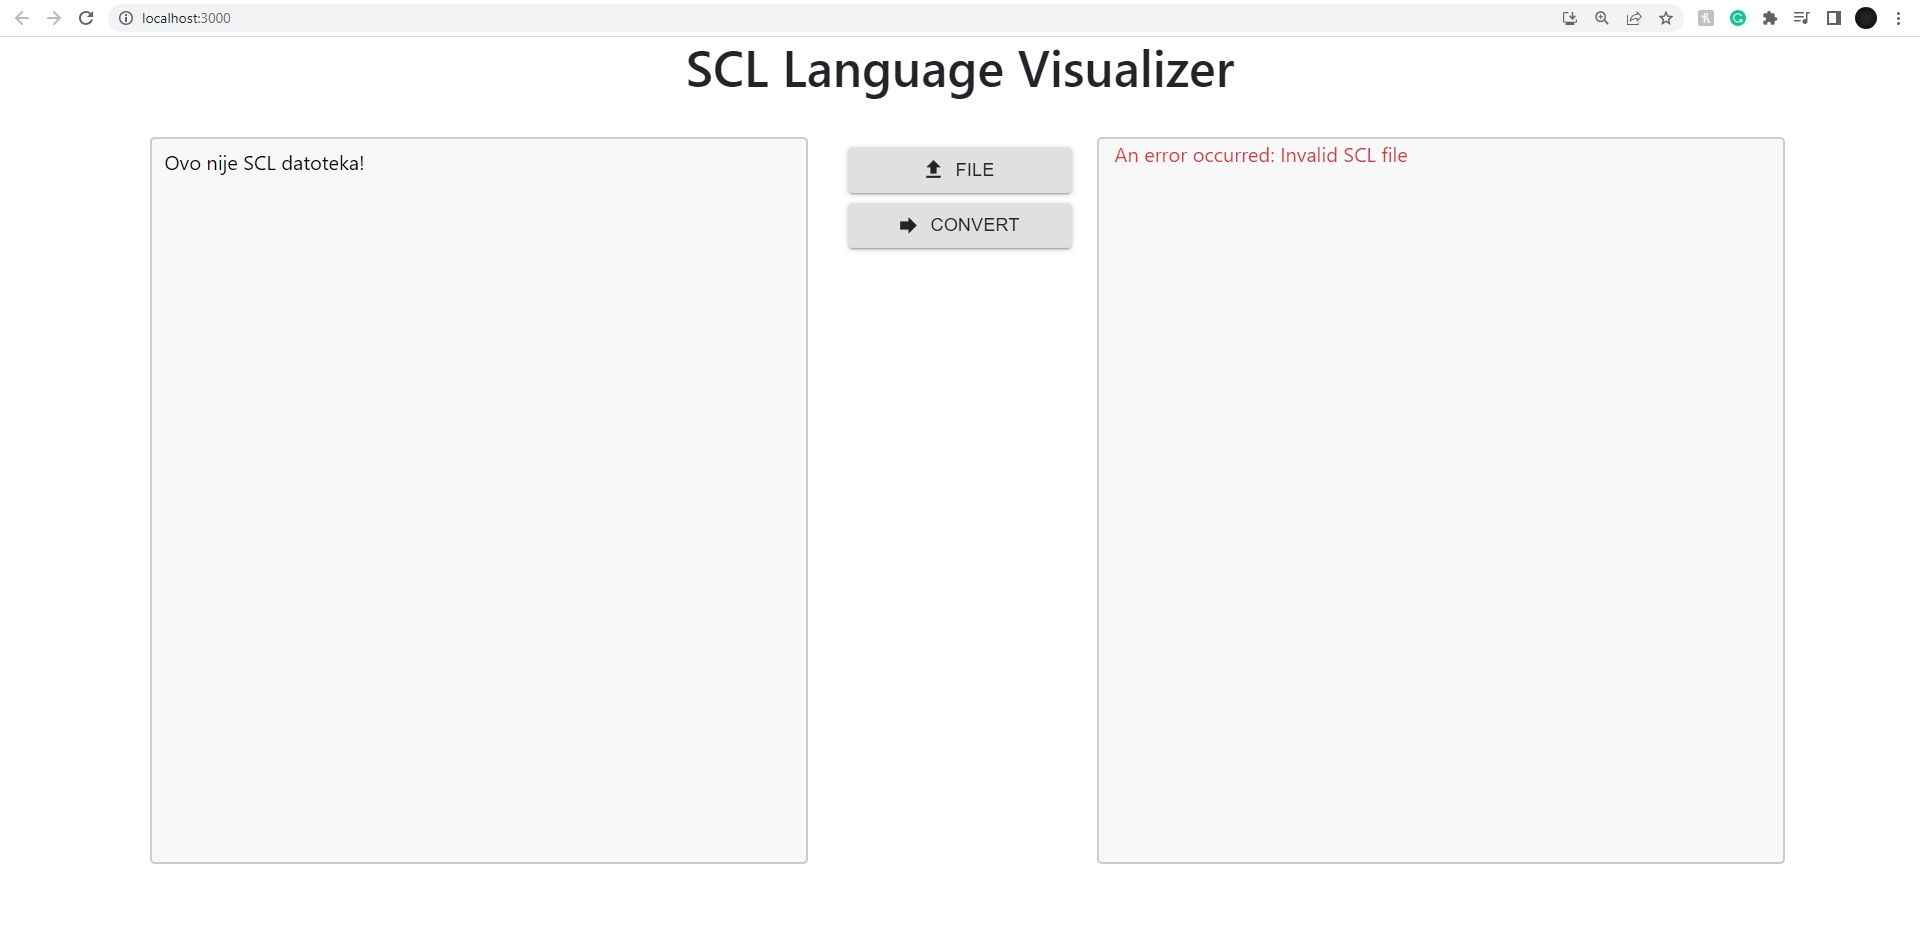
\includegraphics[width=\textwidth]{img/SCL-Visualizer-error.jpg}
    \caption{Prikaz pogreške na klijentskoj strani}
    \label{fig:scl-error}
\end{figure}

\chapter{Zaključak}
Ovaj rad proučava IEC 61850 standard te modele podataka, komunikacijske protokole i konfiguracijski SCL jezik koji on definira. Uz rad je i implementiran alat koji vizualizira SCL datoteke

Najteži dio ovog rada bila je dubina samog IEC 61850 standarda i potrebno predznanje da bi se razumjele njegove implikacije. Dokumentacije vezana za IEC 61850 je oskudna što je također otežalo istraživački dio zadatka.

Vizualizator je na kraju ispao dosta jednostavan zbog kompleksnosti SCL jezika, ali čini dobar temelj. Programski kod je organiziran na način koji je lako nadogradiv stoga se mogućnosti vizualizatora mogu proširiti

\bigskip
Za daljnji nastavak ovog rada potrebno je detaljnije proučiti IED konfigurator i konfigurator sustava kako bi se vizualizator mogao proširiti novim mogućnostima.

\bibliography{literatura}
\bibliographystyle{fer}

\begin{sazetak}
Trafostanice su ključni dio elektroenergetskog sustava, a njihova konfiguracija i arhitektura su kritični za sigurnu i pouzdanu dostavu električne energije kućanstvima. Ovaj rad se bavi IEC 61850 standardom koji je pojednostavnio dizajniranje i konfiguriranje trafostanica. IEC 61850 unificira  modele podataka i komunikacijske protokole u trafostanicama te time omogućuje interoperabilnost uređaja različitih proizvođača. Također, uz ovaj rad implementiran je vizualizator konfiguracijskih datoteka pisanih SCL jezikom kojeg definira IEC 61850 standard.

\kljucnerijeci{IEC 61850, automatizacija trafostanice, komunikacijski protokoli, SCL jezik}
\end{sazetak}

\engtitle{Visualization of substation OT elements described using SCL language}
\begin{abstract}
Substations are a key part of the power system and their configuration and architecture are critical for the safe and reliable delivery of electricity to households. This paper focuses on the IEC 61850 standard, which simplified the design and configuration of substations. IEC 61850 unifies data models and communication protocols in substations and thus enables the interoperability of devices between different manufacturers. Also, along with this work, a visualizer of configuration files written in SCL language defined by the IEC 61850 standard was implemented.

\keywords{IEC 61850, substation automation, communication protocols, SCL language}
\end{abstract}

\end{document}
